\chapter[DOE]{Design of Experiments - DOE}

This chapter is devoted to the matter of designing experiments, and follows the lines of \cite{cox_theory_2000}.
A control chart may be seen as an on-line running experiment alerting us when things go sour. 
When designing a product (remember DFSS \ref{sec:dfss}), or one a control chart has signalled an alert, we will want to know what influences our production, and how to optimize it.
In our SPC terminology, we will want to know what are the \emph{causal} \emph{effects} of our \emph{controllable inputs} (or \emph{factors}), on our \emph{CTQ} (or \emph{response}). 
The theory of discovering these effects is the theory of \emph{design of experiments} (DOE).
Its goal is to \emph{screen} factors with no effect, to estimate effect sizes, and find optimal factor-level combinations; all these as efficiently as possibly.



Roughly speaking, the challenges in designing good experiment are:
\begin{enumerate}
\item Efficiency: extract the most information per sample. 
\item Signal to noise: remove variability that might mask factor effects.
\item Bias: avoid uncontrolled factor-effects from being ``absorbed'' into controlled factor effects.
\end{enumerate}





Before we dig in, several matters should be emphasized:
\begin{description}
\item [Randomization] Randomization is fundamental to our purpose. This because the idea of an \emph{effect} implies causality. Any inference we make, is causal, which is the inference we need for controlling a process.
It is the mechanism of randomization, that allows us to conclude that inferred correlations are causal, and not merely statistical.
For a treatment of causal inference in \emph{observational data}, i.e., without randomization, see \cite{rosenbaum_observational_2002}.

\item [Pre-experiment] In this text we take it for granted that the purpose of the experiment is well known, and the candidate factors defined. We are fully aware, as should be the reader, that in application this is a non-trivial luxury. Indeed, a lot of planning, and domain-knowledge go into the selection of factors, their candidate levels, etc.

\item [Power Analysis] Part of the pre-experiment may include a power analysis. The pre-experiment power analysis will typically be very approximate, and rely on many assumptions. It is still important, as it gives an idea of the feasibility of an experiment, and avoids wasting resources.
\end{description}



\begin{remark}[Analysis of Experimental Data]
In this text, we only discuss the \textbf{design} of the experiment, and not the \textbf{analysis} of the data.
This is a non-standard choice as DOE is typically presented alongside the \emph{analysis of variance} (ANOVA) analysis framework.\marginnote{ANOVA}
We decouple the two since: 
(a) \cite{cox_theory_2000} do so, 
(b) there are two different thing, 
(c) the language of ANOVA may be replaced, as it often is, by the language of \emph{linear models}, \emph{mixed models}, \emph{variance components}, and possibly others. 
There is a vast literature focusing on the analysis method. \marginnote{Linear Models, \\ GLM, \\ Mixed Models, Variance Components}
If asked, this author may recommend \cite{hocking_analysis_1985}, which presents both the ANOVA terminology, and the linear models terminology.
That book, however, may be hard to come by, so feel free to ask me for other references is required.
\end{remark}





\section{Terminology}
Compiled from \cite{mason_statistical_2003}. Many, if not most of the following terms, originate in R.A. Fisher's seminal book ``The Design of Experiments'' \citep{fisher_design_1960}. As usual, when old ideas get new names, we try to emphasize this in the text.



\begin{description}

\item [Experimental Unit]  Entity on which a measurement or an observation is made;
sometimes refers to the actual measurement or observation.
\item [Homogenous Experimental Unit] Units that are as uniform as possible on all characteristics that could affect the response.

\item [Factors]  A controllable experimental variable that is thought to influence the response. In the language of SPC: \emph{a controllable input}.

\item [Level] Specific value of a factor.

\item[Treatment] The particular factor-level combination applied to an experimental unit. \Aka \emph{manipulation}.

\item [Factor Encodings] The numerical encoding of factor levels.
Two level factor encodings include:
\begin{enumerate}
\item Effect coding: where levels are encoded with $-1,1$ returning orthogonal design matrices for balanced designs.
\item Dummy coding: where levels are encoded with $0,1$ returning easily interpretable coefficients.
\end{enumerate}

\item [Experimental Region] All possible factor–level combinations for which experimentation is possible. \Aka \emph{factor space}.

\item [Design Matrix] A matrix description of an experiment that is useful for constructing and analyzing experiments.

\item [Response] The CTQ.

\item [Main Effect] Change in the expected response between two factor–levels.  

\item [Interaction] Existence of joint factor effects in which the effect of each factor depends on the levels of the other factors.

\item [Replication] Repetition of an entire experiment or a portion of an experiment under two or more sets of conditions.

\item [Covariate]  An uncontrollable variable that influences the response but is
unaffected by any other experimental factors.

\item [Design]  Complete specification of experimental test runs, including blocking, randomization, repeat tests, replication, and the assignment of factor–level combinations to experimental units.

\item [Blocking]  Blocking, or \emph{grouping}, is an experimental design technique that removes excess variation by grouping experimental units or test runs so that those units or test runs within a block are more homogeneous than those in different blocks.

\item [Confounding] When the design is such that several effects cannot be told apart. \Aka \emph{aliasing}.

\item [Repeat Tests] Two or more observations that have the same levels for all the factors.

\item [Balance] Some symmetry in the combinatorial design of the experiment. In its simplest interpretation, a design where an equal number of units is assigned to each treatment.

\item [Orthogonality]  Special simplifications of analysis and achievement of efficiency consequent on such \emph{balance}.
\end{description}







\section{Fully Randomized Designs}
Fully randomized designs are those where we freely (and randomly) assign experimental units to treatments.


\subsection{Full Factorial}
A \emph{full factorial} design is one where all factor-level combinations are tested.
In a \emph{balanced full factorial} design, all factor level combinations undergo the same number of \emph{test repeats}.

By far the most common design, in which $k$ factors have 2 levels, is named a $2^k$-design.
Less common, but not surprisingly, $k$ factors with 3 levels is names $3^k$-design, etc.




\subsubsection{$2^1$ design}
Well, this is your usual A/B test. \marginnote{A/B Testing}
There is not much to be said about the design of such experiments, and the analysis is pretty much your good old t-test.




\subsubsection{$2^k$ design}
Consider two factors denoted $A$ and $B$.
Adopt the effect coding so that we encode their levels by $-1,1$.
The design matrix of a single run is depicted in Figure~\ref{fig:full_factorial} (top right) along with a visualization of the design (top left).
Allowing $n$ observations per condition, the experiment will include $4n$ observations, which will be randomized between conditions.
\begin{figure}[ht]
\centering
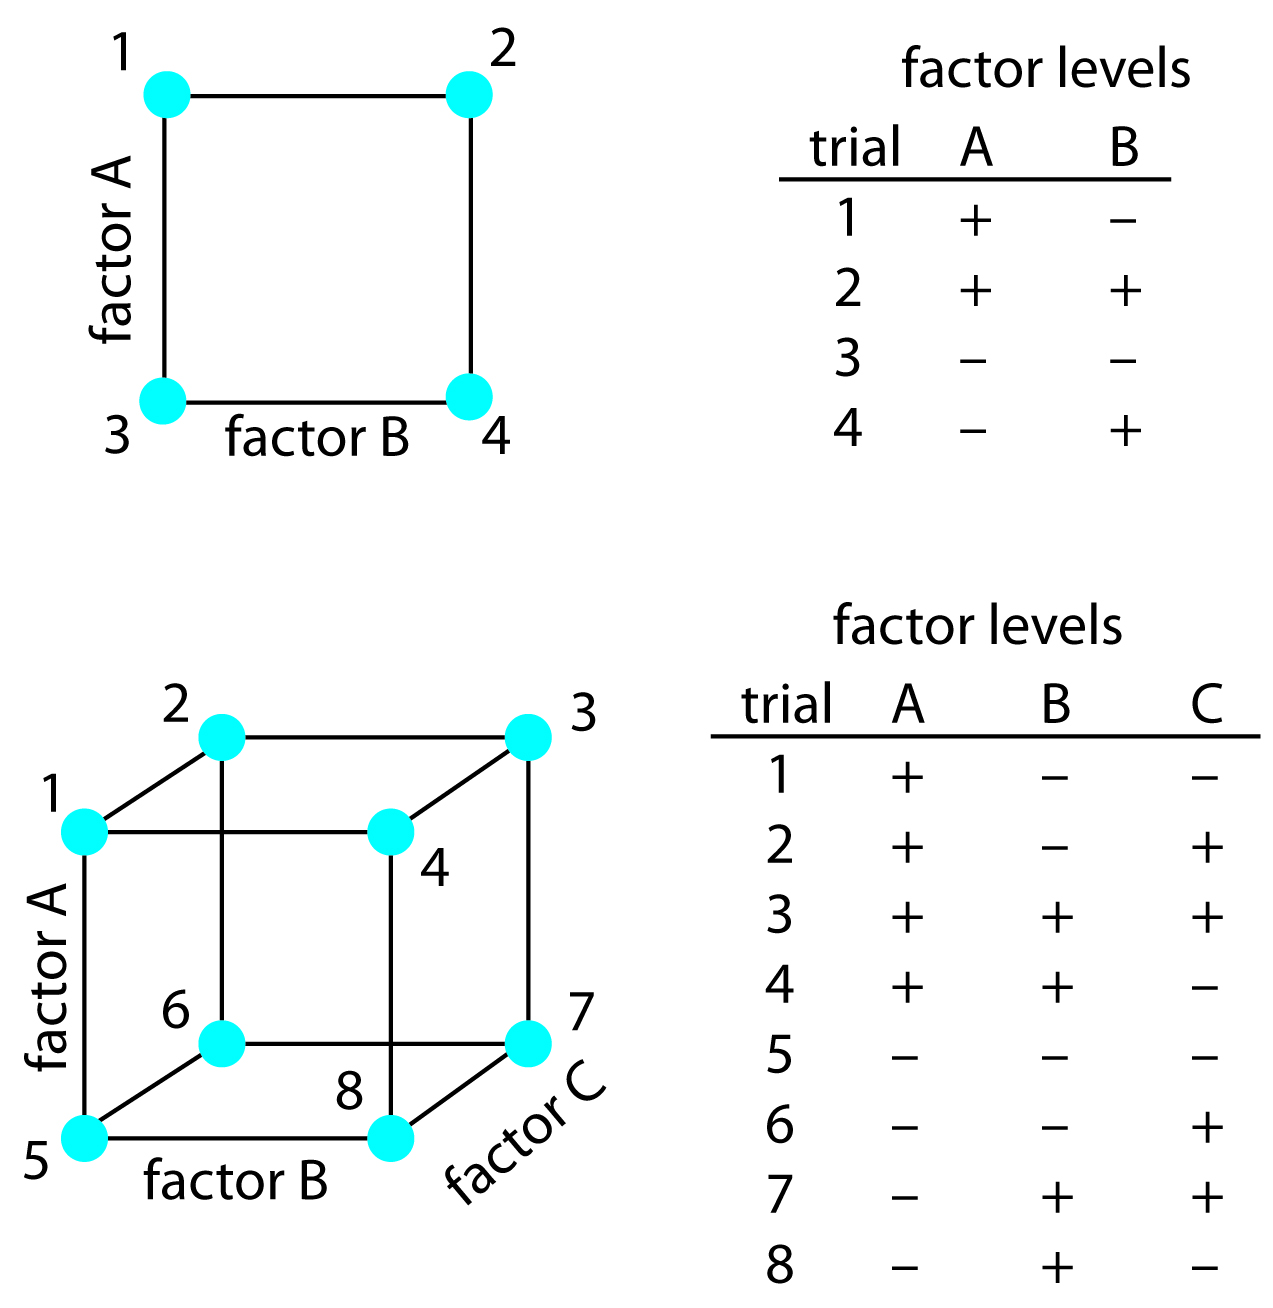
\includegraphics[width=0.7\linewidth, height=0.3\textheight]{art/full_factorial}
\caption{Full factorial designs: $2^2$ and $2^3$. \newline \url{http://chemwiki.ucdavis.edu/Analytical_Chemistry/Analytical_Chemistry_2.0/14_Developing_a_Standard_Method}}
\label{fig:full_factorial}
\end{figure}
With this $2^2$ design, we may recover several effects:
The effect of varying $A$ from $-$ to $+$: the \emph{main effect of $A$} typically denoted $a$. 
The effect of varying $B$ from $-$ to $+$: the \emph{main effect of $B$} typically denoted $b$.  
The effect of varying both $A$ and $B$ from $-$ to $+$. 
We denote the expected response at $A=-,B=-$ with $\mu_{--}$, and the other conditions respectively.
We denote $ab=\mu_{++}-\mu_{--}-a-b$.
If $ab=0$ we say there is \emph{no interaction}.
If $ab \neq 0$, it means that the effect of $A$ depends on the state of $B$, or conversely, that the effect of $B$ depends on the state of $A$.  In short, if $ab \neq 0$ we say there is an \emph{interaction} between $A$ and $B$. \marginnote{Interaction}

Slightly intruding into the realm of data analysis, a visualization of interactions is known as the \emph{interaction plot}, depicted in Figure~\ref{fig:interaction_plot}. 
The upper left panel demonstrates a lack of interaction (think why), while the upper right panel depicts an interaction.
\begin{figure}[ht]
\centering
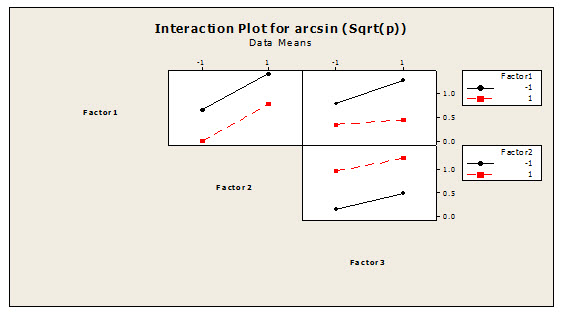
\includegraphics[width=0.3\textheight]{art/attribute_doe_interaction_plot}
\caption{Interactions plot. \newline \url{http://blog.minitab.com/blog/statistics-in-the-field/optimizing-attribute-responses-using-design-of-experiments-doe-part-2}}
\label{fig:interaction_plot}
\end{figure}



\begin{remark}[Intermediate Factor Levels]
In a $2^k$ design, a factor may actually be a continuous controllable input which was restricted to two values for convenience. 
After estimating the effect of the factor, we may want to know what would the effect have been, were we to set it on some intermediate level.
It is customary to assume that a main effect acts linearly in-between experimental conditions, yet you should remember that there is nothing in the data to support this.
For a more rigorous approach, see the Response Surface Methodology section (\ref{sec:response_surface}).
\end{remark}



\subsubsection{$3^k$ Designs}
I think that the name $3^k$ design is rather self explanatory.
Then again, more than $2$ levels are rarely treated as factorial experiments. 
This is because $3$ level factors typically appear when aiming at optimizing the factor combination, for which the \emph{response surface} methodology of Section~\ref{sec:response_surface} is more economical.




\subsection{Fractional Factorial}
The full factorial designs are the simplest designs to setup and interpret. 
A major drawback, are the resources required when $k$ is large. 
This is where the \emph{fractional factorial}, or \emph{partial factorial} designs kick in.
The fundamental idea is to design a full factorial, but skip a couple experimental conditions. 


\begin{example}[From $2^2$ to $2^{(2-1)}$]
\label{eg:fractional_factorial}
As a first example, we will try to save some time and money by eliminating particular conditions of the $2^2$ design in Figure~\ref{fig:full_factorial}.
As the name may suggest, a $2^{2-1}$ design, has $2$ experimental conditions in each run. 
There are thus $\binom{4}{2}=6$ possible eliminations.
\begin{table}[ht]
\begin{tabular}{|p{2.5cm}|p{10cm}|}
\hline Elimination &  Problem \\ 
\hline
\hline 1,2 &  No information on $a$. \\ 
\hline 1,3 &  No information on $b$.\\ 
\hline 1,4 &  $a$ aliased with $b$ aliased with $ab$. \\ 
\hline 2,3 &  $a$ aliased with $b$ aliased with $ab$. \\ 
\hline 2,4 &  No information on $b$. \\ 
\hline 3,4 &  No information on $a$.\\ 
\hline 
\end{tabular} 
\label{tab:partial_factorial}
\caption{Aliasing in a $2^{2-1}$ design: All possible eliminations from the $2^2$ design that lead to a $2^{2-1}$ design.}
\end{table}
\end{example}

The lesson from Example~\ref{eg:fractional_factorial} is that in a fractional factorial our savings in time and money, come at the cost of the information that can be drawn from the experiment.
The idea behind partial factorial experiments, is that by an informed choice of the conditions skipped, we can choose what information to give up. The information lost, is known as the \emph{alias structure}.\marginnote{Alias Structure}

In practice, we will rarely do the actual elimination of conditions, but rather to pre-selected designs. 
Table~\ref{tab:partial_factorial_ii}, generated with the \rcode{FrF2()} in the \rcode{FrF2} \R package, is an optimal $2^{3-1}$ design.
Using the \rcode{design.info()} function of that same package, we know that the aliasing structure of this design is
$a=bd=ce, b=ad, c=ae, d=ab, e=ac$.
We will not do into the details of how the aliasing structure is computed. 

\begin{table}[ht]
\centering
\begin{tabular}{rrrrrr}
  \hline
 & A & B & C & D & E \\ 
  \hline
1 & -1 & 1 & -1 & -1 & 1 \\ 
  2 & 1 & -1 & 1 & -1 & 1 \\ 
  3 & -1 & -1 & -1 & 1 & 1 \\ 
  4 & -1 & 1 & 1 & -1 & -1 \\ 
  5 & -1 & -1 & 1 & 1 & -1 \\ 
  6 & 1 & 1 & 1 & 1 & 1 \\ 
  7 & 1 & -1 & -1 & -1 & -1 \\ 
  8 & 1 & 1 & -1 & 1 & -1 \\ 
   \hline
\end{tabular}
\label{tab:partial_factorial_ii}
\caption{$2^{5-2}$ design.}
\end{table}


As we have already seen, there are $\binom{2^k}{2^{k-p}}$ possible eliminations that convert a $2^k$ design to a $2^{k-p}$ design.
\begin{definition}[Resolution of a Design]
We call the \emph{resolution of the design}, the lowest order effect that is aliased. 
\end{definition}
In Table~\ref{tab:partial_factorial_ii}, the resolution is 1, making it a rather unattractive design. 
Resolutions below 3 typically considered not informative, and above 5, considered wasteful.


\begin{extra}[Minimal Aberration]
If you want to learn how are optimal fractional factorial designs selected, ask me, or Google, for references on \emph{minimal aberration}.
\end{extra}







\section{Controlling Variability Sources}
The idea that random samples come with variability, or noise, should not be new to the reader (but see Extra~\ref{extra:pac_learning} below.)
In this section, we will try to decompose the noise into it sources, or \emph{variance components}, and learn several techniques to reduce the noise sources.
Starting with a motivating example.

\begin{example}[Movie Ratings]
\label{eg:variance_components}
Consider the problem of ranking movies along their rating.
For this purpose, individuals are asked to rate each movie they have seen.
A movie's rating is thus influenced by several factors:
the movie's quality, 
the viewer's strictness, 
the viewer's affinity to that type of movie,
the viewer's mood at the time of watching,
other factors.
How can we accurately rate a movie, in the presence of these variance components?
The movie's quality is a controllable input, thus a factor.
The viewer's strictness is not controllable, but observable, thus may be introduced as a covariate.
The viewer's affinity to that type of movie is an interaction, since both movie type and viewer, are observable.
The viewer's mood is unobservable, we would thus like the viewer to watch as many movies as possible under similar circumstances. Put differently, we would like to \emph{group}, or \emph{block} the time of watching. 
Any other variance source, will be captured by the error term of the model. 
\end{example}

Example~\ref{eg:variance_components} teaches us that by an informed experimental design and analysis, we may reduce noise. Either by moving it to the signal (with covariates), or by removing it (with blocking).
These are the ideas discussed in this section.


\begin{extra}[PAC learning]
\label{extra:pac_learning}
It may be shocking for a statistician, but not all data is noisy.
Try reading about \emph{PAC learning} in the machine learning literature for a counter example.
\end{extra}




\subsection{Gage R\&R Studies}
R\&R stands for \emph{repeatability} and \emph{reproducibility}.
In the context of quality control\footnote{Beware that these words may be used with different meanings by different communities.} repeatability is the variability under repeated measurement, and reproducibility is the variability when the same measurement is performed elsewhere (different lab, technician, etc.).
Gage R\&R experiments consist of performing several \emph{repeat tests}, and different replications, in order to assess R\&R, which can be thought of the variance components attributable inherent to the measurement process.




\subsection{Randomized Block Designs}


\subsubsection{Randomized Complete Block Designs - RCB}
In the simplest case, known awe first block, or group, observations and we then (randomly) assign them to conditions.
If we have $n_c$ experimental conditions, we naturally need blocks of $n_c$ experimental units for a \emph{balanced design}.
The first problem with complete block designs is thus obvious- we may not have $n_c$ observations per block.
The second problem with RCBs is that it typically deals with a single variability source. 
In the movie ranking example (\ref{eg:variance_components}), blocking was along time. 
Clearly time is just a proxy of the viewer's mood. 
If mood is not continuous in time (he got an agitating phone call), then we would need a more elaborate blocking scheme.


\subsubsection{Incomplete Block Designs}
Incomplete block designs arise where there are not enough observations per block to be (randomly) assigned to the $n_c$ experimental conditions.
One natural approach, is to reduce the number of conditions. 
[TODO: balanced incomplete factorial]


\subsubsection{Latin Square Design}
To demonstrate the idea of a Latin-Square design, we revert to an agricultural example, where the whole blocking theory began.

\begin{example}[Agricultural Yield Study]
\label{eg:latin_square}
Consider an farmer growing corn.
He wishes to study the effect of $7$ candidate fertilizers (single factor with $7$ levels).
He is aware that the location of the plot may affect yield, due to slightly different sunlight, irrigation, altitude, etc.
He thus assumes he has to deal with two extra variance sources: row and column of the plot. 
He could treat the row and column as two factors, with $7$ levels each, be he does not care to estimate the row/column effect, but merely to avoid bias.
He will thus try to look for an allocation of fertilizer to rows and columns so that any row/column effect will be averaged out.
The Latin Square design of Table~\ref{tab:latin_square} does just that.
\end{example}
\begin{table}[ht]
\centering
\begin{tabular}{rlllllll}
  \hline
 & 1 & 2 & 3 & 4 & 5 & 6 & 7 \\ 
  \hline
1 & 1 & 2 & 3 & 4 & 5 & 6 & 7 \\ 
  2 & 2 & 3 & 4 & 5 & 6 & 7 & 1 \\ 
  3 & 3 & 4 & 5 & 6 & 7 & 1 & 2 \\ 
  4 & 4 & 5 & 6 & 7 & 1 & 2 & 3 \\ 
  5 & 5 & 6 & 7 & 1 & 2 & 3 & 4 \\ 
  6 & 6 & 7 & 1 & 2 & 3 & 4 & 5 \\ 
  7 & 7 & 1 & 2 & 3 & 4 & 5 & 6 \\ 
   \hline
\end{tabular}
\label{tab:latin_square}
\caption{Latin Square: A $7$-factor latin square, generated with the \rcode{MOLS()} function of the \rcode{crossdes} \R package.
The number in each cell denotes the treatment (the fertilizer in Example~\ref{eg:latin_square}).}
\end{table}

\subsubsection{Extensions of the Latin Square}
\begin{enumerate}
\item \textbf{Latin Hypercube}: When balancing more than two factors (such as row/column), we will call upon \emph{latin hypercube designs}.
\item \textbf{Greco-Latin Square}: A latin-hypercube with three factors. 
\end{enumerate}



\subsubsection{Crossover Design}
Lets return to the movie rating example (\ref{eg:variance_components}).
We can easily agree that tastes may vary considerably between individuals. 
We would like to balance individuals' tastes.
As previously mentioned, we could opt for a blocking strategy so that we cancel within-subject variability.
Alternatively, we may balance the viewing periods over subjects. 
This will not remove within-subject variability, but it will avoid a ``mood bias''.

In \emph{crossover designs}, or \emph{crossover trials}, each unit undergoes several treatments.
Preferably, the design is balanced so that each unit undergoes all treatments.
You are certainly familiar with the idea, since the paired t-test from your introductory statistical courses is just a crossover deign with two treatments.

In a \emph{fully randomized crossover design}, each unit is randomly allocated to a sequence of treatments.
If units are suspceted to be non-homogenous, then we may block, and assign full blocks to sequences.
\begin{table}[ht]
\centering
\begin{tabular}{rlll}
  \hline
 & 1 & 2 & 3 \\ 
  \hline
1 & 1 & 2 & 3 \\ 
  2 & 2 & 3 & 1 \\ 
  3 & 3 & 1 & 2 \\ 
  4 & 1 & 3 & 2 \\ 
  5 & 2 & 1 & 3 \\ 
  6 & 3 & 2 & 1 \\ 
   \hline
\end{tabular}
\label{tab:crossover}
\caption{Crossover design: a balanced sequence of administration of $3$ treatments, generated with the \rcode{des.MOLS()} function of the \rcode{crossdes} \R package. }
\end{table}


\begin{remark}[Crossed Treatments]
Both crossover designs and full factorial designs are \emph{crossed} in that all factor combinations are sampled. 
The difference is that in a full-factorial, a factor combination is applied simultaneously to an experiment unit, and in a crossover design, the application is sequential.[TODO: cite cambridge dictionary of statistics]
\end{remark}



\subsection{Nested Designs}
Until now, whenever you had several factors, and resources permit, we aimed at \emph{crossing} all factors levels, so that in the analysis stage we may recover information on all main-effects, and interactions.
There are cases, however, where crossing factors does not make any sense.
This is the idea of \emph{nested designs}, \aka \emph{hirarchial design}, demonstrated in the following example.\marginnote{Hirarchial Design}

\begin{example}[TODO]
content...
\end{example}


\subsubsection{Nested and Crossed Designs}

\subsubsection{Split Plot Designs}




\subsection{Process Improvement Designs}



\subsubsection{Taguchi's Robust Design Approach}



\section{Continuous Factors}



\subsection{Response Surface Methdology}
\label{sec:response_surface}

\subsubsection{Central Composite Design}

\subsubsection{Box-Behnken Design}

\subsection{Optimal Designs}

\subsubsection{A optimality}
\subsubsection{B optimality}
\subsubsection{C optimality}
\subsubsection{D optimality}




\section{Sequential Designs}
% Mark Vandelmeulenbruke

\subsubsection{Active Learning}


\subsubsection{MultiArmed Bandits}




\section{Adaptive Designs}



\section{Computer Experiments}

